\documentclass[12pt,a4paper]{article}
	%[fleqn] %%% --to make all equation left-algned--

% \usepackage[utf8]{inputenc}
% \DeclareUnicodeCharacter{1D12A}{\doublesharp}
% \DeclareUnicodeCharacter{2693}{\anchor}
% \usepackage{dingbat}
% \DeclareRobustCommand\dash\unskip\nobreak\thinspace{\textemdash\allowbreak\thinspace\ignorespaces}
\usepackage[top=2in, bottom=1in, left=1in, right=1in]{geometry}
%\usepackage{fullpage}

\usepackage{fancyhdr}\pagestyle{fancy}\rhead{Stephanie Wang}\lhead{EE236B homework 2}

\usepackage{amsmath,amssymb,amsthm,amsfonts,microtype,stmaryrd}
	%{mathtools,wasysym,yhmath}

\usepackage[usenames,dvipsnames]{xcolor}
\newcommand{\blue}[1]{\textcolor{blue}{#1}}
\newcommand{\red}[1]{\textcolor{red}{#1}}
\newcommand{\gray}[1]{\textcolor{gray}{#1}}
\newcommand{\fgreen}[1]{\textcolor{ForestGreen}{#1}}

\usepackage{mdframed}
	%\newtheorem{mdexample}{Example}
	\definecolor{warmgreen}{rgb}{0.8,0.9,0.85}
	% --Example:
	% \begin{center}
	% \begin{minipage}{0.7\textwidth}
	% \begin{mdframed}[backgroundcolor=warmgreen, 
	% skipabove=4pt,skipbelow=4pt,hidealllines=true, 
	% topline=false,leftline=false,middlelinewidth=10pt, 
	% roundcorner=10pt] 
	%%%% --CONTENTS-- %%%%
	% \end{mdframed}\end{minipage}\end{center}	

\usepackage{graphicx} \graphicspath{{}}
	% --Example:
	% \includegraphics[scale=0.5]{picture name}
%\usepackage{caption} %%% --some awful package to make caption...

%\usepackage{hyperref}\hypersetup{linktocpage,colorlinks}\hypersetup{citecolor=black,filecolor=black,linkcolor=black,urlcolor=black}

%%% --Text Fonts
%\usepackage{times} %%% --Times New Roman for LaTeX
%\usepackage{fontspec}\setmainfont{Times New Roman} %%% --Times New Roman; XeLaTeX only

%%% --Math Fonts
\renewcommand{\v}[1]{\ifmmode\mathbf{#1}\fi}
%\renewcommand{\mbf}[1]{\mathbf{#1}} %%% --vector
%\newcommand{\ca}[1]{\mathcal{#1}} %%% --"bigO"
%\newcommand{\bb}[1]{\mathbb{#1}} %%% --"Natural, Real numbers"
%\newcommand{\rom}[1]{\romannumeral{#1}} %%% --Roman numbers

%%% --Quick Arrows
\newcommand{\ra}[1]{\ifnum #1=1\rightarrow\fi\ifnum #1=2\Rightarrow\fi\ifnum #1=3\Rrightarrow\fi\ifnum #1=4\rightrightarrows\fi\ifnum #1=5\rightleftarrows\fi\ifnum #1=6\mapsto\fi\ifnum #1=7\iffalse\fi\fi\ifnum #1=8\twoheadrightarrow\fi\ifnum #1=9\rightharpoonup\fi\ifnum #1=0\rightharpoondown\fi}

%\newcommand{\la}[1]{\ifnum #1=1\leftarrow\fi\ifnum #1=2\Leftarrow\fi\ifnum #1=3\Lleftarrow\fi\ifnum #1=4\leftleftarrows\fi\ifnum #1=5\rightleftarrows\fi\ifnum #1=6\mapsfrom\ifnum #1=7\iffalse\fi\fi\ifnum #1=8\twoheadleftarrow\fi\ifnum #1=9\leftharpoonup\fi\ifnum #1=0\leftharpoondown\fi}

%\newcommand{\ua}[1]{\ifnum #1=1\uparrow\fi\ifnum #1=2\Uparrow\fi}
%\newcommand{\da}[1]{\ifnum #1=1\downarrow\fi\ifnum #1=2\Downarrow\fi}

%%% --Special Editor Config
\renewcommand{\ni}{\noindent}
\newcommand{\onum}[1]{\raisebox{.5pt}{\textcircled{\raisebox{-1pt} {#1}}}}

\newcommand{\claim}[1]{\underline{``{#1}":}}

\renewcommand{\l}{\left}\renewcommand{\r}{\right}

\newcommand{\casebrak}[2]{\left \{ \begin{array}{l} {#1}\\{#2} \end{array} \right.}
%\newcommand{\ttm}[4]{\l[\begin{array}{cc}{#1}&{#2}\\{#3}&{#4}\end{array}\r]} %two-by-two-matrix
%\newcommand{\tv}[2]{\l[\begin{array}{c}{#1}\\{#2}\end{array}\r]}

\def\dps{\displaystyle}

\let\italiccorrection=\/
\def\/{\ifmmode\expandafter\frac\else\italiccorrection\fi}


%%% --General Math Symbols
\def\bc{\because}
\def\tf{\therefore}

%%% --Frequently used OPERATORS shorthand
\newcommand{\INT}[2]{\int_{#1}^{#2}}
% \newcommand{\UPINT}{\bar\int}
% \newcommand{\UPINTRd}{\overline{\int_{\bb R ^d}}}
\newcommand{\SUM}[2]{\sum\limits_{#1}^{#2}}
\newcommand{\PROD}[2]{\prod\limits_{#1}^{#2}}
\newcommand{\CUP}[2]{\bigcup\limits_{#1}^{#2}}
\newcommand{\CAP}[2]{\bigcap\limits_{#1}^{#2}}
% \newcommand{\SUP}[1]{\sup\limits_{#1}}
% \newcommand{\INF}[1]{\inf\limits_{#1}}
\DeclareMathOperator*{\argmin}{arg\,min}
\DeclareMathOperator*{\argmax}{arg\,max}
\newcommand{\pd}[2]{\frac{\partial{#1}}{\partial{#2}}}
\def\tr{\text{tr}}

\renewcommand{\o}{\circ}
\newcommand{\x}{\times}
\newcommand{\ox}{\otimes}

\newcommand\ie{{\it i.e.}}
\newcommand\dom{\mathbf{dom}}

%%% --Frequently used VARIABLES shorthand
\def\R{\ifmmode\mathbb R\fi}
\def\N{\ifmmode\mathbb N\fi}
\renewcommand{\O}{\mathcal{O}}

\newcommand{\dt}{\Delta t}
\def\vA{\mathbf{A}}
\def\vB{\mathbf{B}}\def\cB{\mathcal{B}}
\def\vC{\mathbf{C}}
\def\vD{\mathbf{D}}
\def\vE{\mathbf{E}}
\def\vF{\mathbf{F}}\def\tvF{\tilde{\mathbf{F}}}
\def\vG{\mathbf{G}}
\def\vH{\mathbf{H}}
\def\vI{\mathbf{I}}\def\cI{\mathcal{I}}
\def\vJ{\mathbf{J}}
\def\vK{\mathbf{K}}
\def\vL{\mathbf{L}}\def\cL{\mathcal{L}}
\def\vM{\mathbf{M}}
\def\vN{\mathbf{N}}\def\cN{\mathcal{N}}
\def\vO{\mathbf{O}}
\def\vP{\mathbf{P}}
\def\vQ{\mathbf{Q}}
\def\vR{\mathbf{R}}
\def\vS{\mathbf{S}}
\def\vT{\mathbf{T}}
\def\vU{\mathbf{U}}
\def\vV{\mathbf{V}}
\def\vW{\mathbf{W}}
\def\vX{\mathbf{X}}
\def\vY{\mathbf{Y}}
\def\vZ{\mathbf{Z}}

\def\va{\mathbf{a}}
\def\vb{\mathbf{b}}
\def\vc{\mathbf{c}}
\def\vd{\mathbf{d}}
\def\ve{\mathbf{e}}
\def\vf{\mathbf{f}}
\def\vg{\mathbf{g}}
\def\vh{\mathbf{h}}
\def\vi{\mathbf{i}}
\def\vj{\mathbf{j}}
\def\vk{\mathbf{k}}
\def\vl{\mathbf{l}}
\def\vm{\mathbf{m}}
\def\vn{\mathbf{n}}
\def\vo{\mathbf{o}}
\def\vp{\mathbf{p}}
\def\vq{\mathbf{q}}
\def\vr{\mathbf{r}}
\def\vs{\mathbf{s}}
\def\vt{\mathbf{t}}
\def\vu{\mathbf{u}}
\def\vv{\mathbf{v}}\def\tvv{\tilde{\mathbf{v}}}
\def\vw{\mathbf{w}}
\def\vx{\mathbf{x}}\def\tvx{\tilde{\mathbf{x}}}
\def\vy{\mathbf{y}}
\def\vz{\mathbf{z}}

%%% --Numerical analysis related
%\newcommand{\nxt}{^{n+1}}
%\newcommand{\pvs}{^{n-1}}
%\newcommand{\hfnxt}{^{n+\frac12}}

%%%%%%%%%%%%%%%%%%%%%%%%%%%%%%%%%%%%%%%%%%%%%%%%%%%%%%%%%%%%%%%%%%%%%%%%%%%%%%%%%%%%%%%%%%%%%%%%%%%%%%%%%%%%%%%%%%%%%%%%%%%%%%%%%%%%%%%%%%%%%%%%%%%%%%%%%%%%%%%%%%%%%%%%%%%%%%%%%%%%%%%%%%%%%%%%%%%%%%
\begin{document}
\subsubsection*{Exercise 2.37 [Boyd \& Vandenberghe, 2004]}
\noindent {\it Nonnegative polynomials and Hankel LMIs.} Let $K_{pol}$ be the set of (coefficients of) non-negative polynomials of degree $2k$ on $\R$:
$$K_{pol} = \{ x\in \R^{2k+1} \mid x_1 + x_2t + x_3t^2 + \cdots + x_{2k+1}t^{2k} \geq 0 \forall t\in\R\}$$
(a) Show that $K_{pol}$ is a proper cone. \\
(b) A basic result states that a polynomial of degree $2k$ is nonnegative on $\R$ if and only if it can be expressed as the sum of squares of two polynomials of degree $k$ or less. In other words, $x\in K_{pol}$ if and only if the polynomial 
$$p(t) = x_1 + x_2t + x_3t^2 + \cdots + x_{2k+1}t^{2k}$$
can be expressed as 
$$p(t) = r(t)^2 + s(t)^2,$$
where $r$ and $s$ are polynomials of degree $k$. \\
Use this result to show that 
$$K_{pol} = \l\{x\in\R^{2k+1} \mid x_i = \SUM{m+n=i+1}{} Y_{mn}, Y \in \vS^{k+1}_+  \r\}$$
In other words, $p(t) = x_1 + x_2 t + x_3 t^2 + \cdots + x_{2k+1}t^{2k}$ is nonnegative if and only if there exists a matrix $Y\in\vS^{k+1}_+$ such that 
\begin{align*}
x_1 &= Y_{11}\\
x_2 &= Y_{12} + Y_{21} \\
x_3 &= Y_{13}+Y_{22}+Y_{31}\\
&\vdots\\
x_{2k+1} &= Y_{k+1,k+1}.
\end{align*}
(c) Show that $K_{pol}^\ast = K_{han}$ where 
$$K_{han} = \{z\in\R^{2k+1} \mid H(z) \succeq 0\}$$
and 
$$H(z) = \l[\begin{array}{cccccc}
z_1 & z_2 & z_3 & \cdots & z_k & z_{k+1}\\
z_2 & z_3 & z_4 & \cdots & z_{k+1} & z_{k+2}\\
z_3 & z_4 & z_5 & \cdots & z_{k+2} & z_{k+3}\\
\vdots & \vdots & \vdots & \ddots & \vdots & \vdots\\
z_k & z_{k+1} & z_{k+2} & \cdots & z_{2k-1} & z_{2k}\\
z_{k+1} & z_{k+2} & z_{k+3} & \cdots & z_{2k} & z_{2k+1}
 \end{array}\r]$$
(This is the {\it Hankel matrix} with coefficients $z_1, \cdots, z_{2k+1}$.) \\
(d) Let $K_{mom}$ be the conic hull of the set of all vectors of the form $(1,t,t^2, \cdots, t^{2k})$, where $t\in\R$. Show that $y\in K_{mom}$ if and only if $y_1\geq 0$ and 
$$y = y_1 (1, \vE u, \vE u^2, \cdots , \vE u^{2k})$$
for some random variable u. In other words, the elements of $K_{mom}$ are nonnegative multiples of the moment vectors of all possible distributions on $\R$. Show that $K_{pol} = K_{mom}^\ast$. \\
(e) Combining the results of (c) and (d), conclude that $K_{han} = \mathbf{cl}K_{mom}$. \\
AS an example illustrating the relation between $K_{mom}$ and $K_{han}$, take $k=2$ and $z=(1,0,0,0,1)$. Show that $z\in K_{han}$, $z\notin K_{mom}$. Find an explicit sequence of points in $K_{mom}$ which converge to $z$. \\
\\
{\it Ans:} Here only presents solutions to (b) and (c).\\
(b) Write $r(t) = r_1+r_2t +r_3t^2+\cdots+r_{k+1}t^k$, $s(t) = s_1+s_2t+s_3t^2+\cdots+s_{k+1}s^k$ and the coefficient vectors $r = [r_1, r_2, r_3, \cdots, r_{k+1}], s = [s_1, s_2, s_3, \cdots, s_{k+1}]$, then 
$$r(t) = r^T\l[\begin{array}{c}
1\\
t\\
t^2\\
\vdots\\
t^k\end{array}\r], s(t) = s^T\l[\begin{array}{c}
1\\
t\\
t^2\\
\vdots\\
t^k\end{array}\r]$$
Denote $e(t) = \l[\begin{array}{c}
1\\
t\\
t^2\\
\vdots\\
t^k\end{array}\r]$ to avoid using the exhausting package for arrays; we see 
$$r(t)^2 = e(t)^T r r^T e(t), s(t) = e(t)^T s s^T e(t)$$
Let $R = rr^T, S = ss^T$, due to the structure these two matrices are positive semidefinite. (e.g. for any given $z\in\R^{k+1}$, $z^T R z = (r^T z)^2 \geq 0$. ) Let $Y = R+S \in \vS^{k+1}_+$. (sum of two positive semidefinite matrices is still positive semidefinite. ) It's now evident that 
\begin{align*}
p(t) &= e(t)^T Y e(t) \\
&= \SUM{m,n=1}{k+1} t^{m-1}Y_{mn}t^{n-1} \\
&= \SUM{m,n=1}{k+1} Y_{mn} t^{m+n-2} \\
&= \SUM{j=0}{2k} \l(\SUM{m+n=j+2}{} Y_{mn}\r) t^j
\end{align*}
and 
$$x_{j+1} = \SUM{m+n=j+2}{} Y_{mn}, \mbox{ or, } x_i = \SUM{m+n=i+1}{}Y_{mn}$$
On the other hand, if $x_i = \SUM{m+n=i+1}{}Y_{mn}$ for some $Y\in\vS^{k+1}_+$, then by similar index substitution trick, 
$$p(t) = e(t)^T Y e(t) \geq 0$$
for any $t\in\R$, since $Y$ is positive semidefinite. \\
\\
(c) Note that for $x\in K_{pol}$ that corresponds to $Y(x)\in\vS^{k+1}_+$, 
\begin{align*}
x^Tz & = \SUM{i=1}{2k+1} x_iz_i  \\
&= tr(Y(x)^TH(z))
\end{align*}
Due to the fact that $(\vS^{k+1}_+)^\ast = \vS^{k+1}_+$, we conclude $K_{pol}^\ast = K_{han}$. \qed




\newpage\subsubsection*{Exercise 3.1 [Boyd \& Vandenberghe, 2004]}
\noindent Suppose $f:\R \ra1 \R$ is convex, and $a, b \in \dom f$ with $a<b$. \\
(a) Show that 
$$f(x) \leq \/{b-x}{b-a} f(a) + \/{x-a}{b-a}f(b)$$
for all $x\in[a,b]$. \\
(b) Show that 
$$\/{f(x)-f(a)}{x-a}\leq \/{f(b)-f(a)}{b-a} \leq \/{f(b)-f(x)}{b-x}$$
for all $x\in (a,b)$. Draw a sketch that illustrates this inequality. \\
(c) Suppose $f$ is differentiable. Use the result in (b) to show that 
$$f'(a) \leq \/{f(b)-f(a)}{b-a} \leq f'(b).$$
Note that these inequalities also follow from (3.2):
$$f(b) \geq f(a) + f'(a) (b-a), f(a) \geq f(b)+f'(b)(a-b)$$
(d) Suppose $f$ is twice differentiable. Use the result in (c) to show that $f''(a) \geq 0$ and $f''(b) \geq 0$.\\
\\
{\it Ans:} \\
(a) Let $\theta = \/{b-x}{b-a} \in [0,1]$, then the inequality is nothing but
$$f(\theta a + (1-\theta)b) \leq \theta f(a) + (1-\theta)f(b)$$
(b) The leftmost term is the slope of the secant jointing $(a, f(a)), (x, f(x))$, second $(a, f(a)), (b, f(b))$, and third $(x,f(x)), (b,f(b))$; it suffices to show the slope of secants of the curve is increasing, that is, one equality of the two given ones. Take the inequality in (a) and subtract both sides with $f(a)$
\begin{align*}
f(x) - f(a) &\leq  \l(\/{b-x}{b-a}-1\r) f(a) + \/{x-a}{b-a}f(b)\\
&= -\/{x-a}{b-a}f(a) + \/{x-a}{b-a}f(b)\\
&= \/{x-a}{b-a}(f(b)-f(a)\\
\frac{f(x)-f(a)}{x-a} &\leq \/{f(b)-f(a)}{b-a} \mbox{ \;\;\;\;\;(divide both sides with $x-a$)}
\end{align*}
(c) $f'(a)$ is the limit of LHS (of the inequality from (b)) as $x\ra1 a^+$ and $f'(b)$ RHS as $x\ra1 b^-$. By differentiability, limit taken on single side should gives the derivative. \\
Also by manipulating terms in (3.2) (subtracting $f(a)$ or $f(b)$ and dividing by $b-a$) we can get this inequality too. \\
\\
(d) The inequality $f'(a) \leq f'(b)$ for arbitrary $a$ and $b$ shows the monotonicity of $f'(x)$. By basic calculus we know the derivative of a monotonically increasing function must be nonnegative, that is $f''(x) \geq 0$ for all $x\in(a, b)$. (The proof involves Mean Value Theorem. I can elaborate if required.) \qed







\newpage\subsubsection*{Exercise 3.2 [Boyd \& Vandenberghe, 2004]}
\noindent {\it Level sets of convex, concave, quasiconvex, and quasiconcave functions.} Some level sets of a function $f$ are shown below. The curve labeled 1 shows $\{x \mid f(x) = 1\}$, etc.
\begin{center}
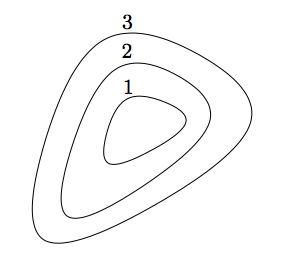
\includegraphics[scale=0.5]{hw2_p32-1.png}
\end{center}
Could $f$ be convex (concave, quasiconvex, quasiconcave)? Explain your answer. Repeat for the level curves shown below. 
\begin{center}
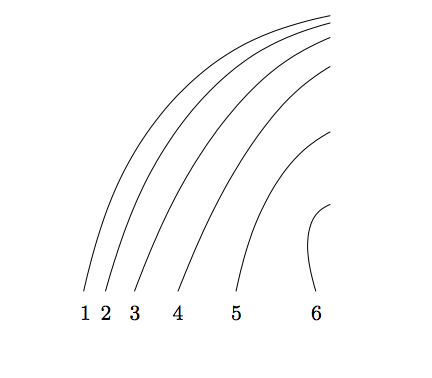
\includegraphics[scale=0.5]{hw2_p32-2.png}
\end{center}
{\it Ans:} From the graphs we can first assert the first function is quasiconvex and second quasiconcave, due to the convexity of the level sets. We can further suggest the first function is convex; picture the epigraph by looking at the level sets, each slide of it looks rather like a parabola. We can't suggest the second function to be concave because the function doesn't seem increasing enough from the upper left corner to the lower left corner, which could make its epigraph non concave. 




\newpage\subsubsection*{Additional Exercise 2.10 [Boyd \& Vandenberghe, 2017]}
\noindent {\it Weighted geometric mean.} The geometric mean $f(x) = (\prod_k x_k)^{1/n}$ with $\dom f = \R^{n}_{++}$ is concave, as shown on page 74. Extend the proof to show that 
$$f(x) = \PROD{k=1}n x_k^{\alpha_k}, \dom f = \R^n_{++}$$
is concave, where $\alpha_k$ are positive numbers with $\sum_k \alpha_k \leq 1$. \\
\\
{\it Ans:} First observe functions $m_k(x_k) = x_k^{\alpha_k}$ are positive (we're assuming $x_k > 0$) and concave since $\alpha_k \in [0, 1]$. ($m_k''(x_k) = -\alpha_k(1-\alpha_k) x_k^{\alpha_k-2} \leq 0$.) \\
Take first derivative of $f$,
$$\nabla f(x) = \l[\begin{array}{c}
\alpha_1x^{\alpha_1-1} \PROD{k\neq 1}{} x_k^{\alpha_k}\\
\alpha_2x^{\alpha_2-1} \PROD{k\neq 2}{} x_k^{\alpha_k}\\
\vdots\\
\alpha_nx^{\alpha_n-1} \PROD{k\neq n}{} x_k^{\alpha_k}\\
\end{array}\r]$$
and then second derivative,
\begin{align*} 
H_f(x) &= \l[\begin{array}{cccc}
\frac{f(x)\alpha_1(\alpha_1-1)}{x_1^2}  & \frac{f(x)\alpha_1\alpha_2}{x_1x_2}  &\cdots & \frac{f(x)\alpha_1\alpha_n}{x_1x_n}   \\
\frac{f(x)\alpha_1\alpha_2}{x_1x_2}  & \frac{f(x)\alpha_2(\alpha_2-1)}{x_2^2}  & \cdots & \\
\vdots & \vdots& \ddots& \\
\frac{f(x)\alpha_1\alpha_n}{x_1x_n}  & & & \frac{f(x)\alpha_n(\alpha_n-1)}{x_n^2} 
\end{array}\r]\\
& =: f(x) A(x)
\end{align*}
Observe that $A(x) = \l[\begin{array}{cccc}
\frac{\alpha_1(\alpha_1-1)}{x_1^2}  & \frac{\alpha_1\alpha_2}{x_1x_2}  &\cdots & \frac{\alpha_1\alpha_n}{x_1x_n}   \\
\frac{\alpha_1\alpha_2}{x_1x_2}  & \frac{\alpha_2(\alpha_2-1)}{x_2^2}  & \cdots & \\
\vdots & \vdots& \ddots& \\
\frac{\alpha_1\alpha_n}{x_1x_n}  & & & \frac{\alpha_n(\alpha_n-1)}{x_n^2} 
\end{array}\r]$ is diagonally dominant with all negative diagonal entries; e.g. for the first column/row
\begin{align*}
|a_{11}| - \SUM{i=2}n |a_{i1}| &= \/{\alpha_1}{x_1^2}\l( (1-\alpha_1) - \alpha_2 - \cdots - \alpha_n \r) \\
&= \/{\alpha_1}{x_1^2}\l(1-\SUM{i=1}n\alpha_i\r) \leq 0
\end{align*}
since by assumption $\sum_i \alpha_i \leq 1$.  \qed




\newpage\subsubsection*{Additional Exercise 5.8 [Boyd \& Vandenberghe, 2017]}
\noindent {\it Least-squares fitting with convex splines. } A {\it cubic spline} (or {\it fourth-order spline}) with breakpoints $\alpha_0, \alpha_1, \cdots, \alpha_M$ (that satisfy $\alpha_0 < \alpha_1 < \cdots < \alpha_M$) is a piecewise-polynomial function with the following properties: \begin{itemize}
\item the function is a cubic polynomial on each interval $[\alpha_i, \alpha_{i+1}]$
\item the function values, and the first and second derivatives are continuous on the interval $(\alpha_0, \alpha_M)$.
\end{itemize}
The figure shows an example of a cubic spline $f(t)$ with $M=10$ segments and breakpoints $\alpha_0=0, \alpha_1 = 1, \cdots, \alpha_{10} = 10$.
\begin{center}
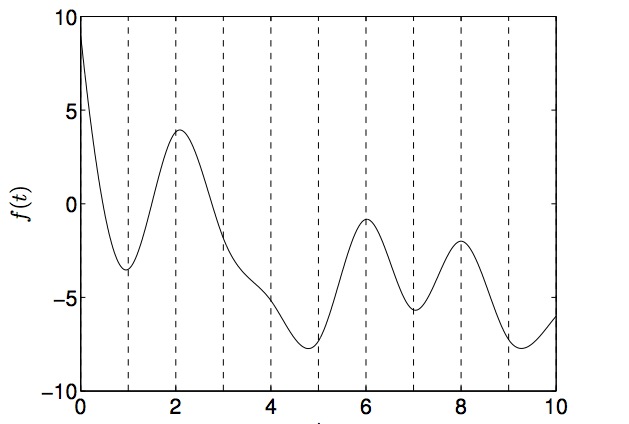
\includegraphics[scale=0.5]{hw2_p58.png}
\end{center}
In approximation problems with splines it is convenient to parametrize a spline as a linear combination of basis functions, called {\it B-splines}. The precise definition of B-splines is not important for our purposes; it is sufficient to know that every cubic spline can be written as a linear combination of $M+3$ cubic B-splines $g_k(t)$, \ie, in the form
$$f(t) = s_1g_1(t) + \cdots + x_{M+3}g_{M+3}(t) = x^T g(t),$$
and that there exist efficient algorithms for computing $g(t) = (g_1(t), \cdots, g_{M+3}(t))$. The next figure shows the 13 B-splines for the breakpoints $0, 1, \cdots, 10$. 
\begin{center}
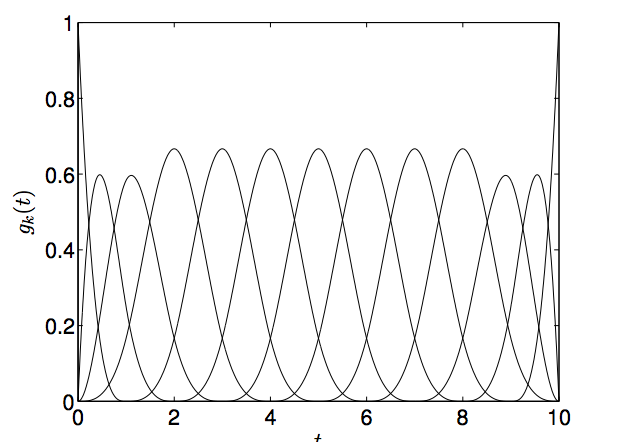
\includegraphics[scale=0.5]{hw2_p58-1.png}
\end{center}
In this exercise we study the problem of fitting a cubic spline to a set of data points, subject to the constraint that the spline is a convex function. Specifically, the breakpoints $\alpha_0, \cdots, \alpha_M$ are fixed, and we are given $N$ data points $(t_k, y_k)$ with $t_k \in [\alpha_0, \alpha_M]$. We are asked to find the convex cubic spline $f(t)$ that minimizes the least squares criterion
$$\SUM{k=1}N (f(t_k)-y_k)^2.$$
We will use B-splines to parametrize $f$, so the variables in the problem are the coefficients $x$ in $f(t) = x^Tg(t)$. The problem can then be written as 
\begin{equation}\label{1}
\begin{array}{ll}
\mbox{minimize}& \SUM{k=1}N \l(x^Tg(t_k)-y_k\r)^2\\
\mbox{subject to}& x^Tg(t) \mbox{ is convex in } t \mbox{ on } [\alpha_0, \alpha_M]
\end{array}\end{equation}
(a) Express problem \eqref{1} as a convex optimization problem of the form
$$\begin{array}{ll}
\mbox{minimize}& \|Ax-b\|^2_2\\
\mbox{subject to}& Gx \preceq h
\end{array}$$
(b) Use CVX to solve a specific instance of the optimization problem in part (a). As in the figures above, we take $M=10$ and $\alpha_0=0, \alpha_1=1, \cdots, \alpha_{10}=10$. \\
Download the Matlab files \texttt{spline\_data.m} and \texttt{bsplines.m}. The first m-file is used to generate the problem data. The command \texttt{[t, y] = spline\_data} will generate two vectors $t, y$ of length $N=51$, with the data points $t_k, y_k$.\\
The second function can be used to compute the B-splines, and their first and second derivatives, at any given point $u\in [0, 10]$. The command \texttt{[g, gp, gpp] = bsplines(u)} returns three vectors of length 13 with elements $g_k(u), g_k'(u)$, and $g_k''(u)$. (The right derivatives are returned for $u=0$, and the left derivatives for $u=10$.)\\
Solve the convex spline fitting problem \eqref{1} for this example, and plot the optimal spline. \\
\\
{\it Ans:} 
(a) Let $a_{ij} = g_j(t_i)$ and $b_i = y_i$ then
\begin{align*}
\SUM{i=1}N (x^T g(t_i) - y_i)^2 & = \SUM{i=1}N \l(\SUM{j=1}{M+3} x_jg_j(t_i) - y_i\r)^2\\
&= \|Ax-b\|_2^2
\end{align*}
where $A = [a_{ij}] \in \R^{N\x(M+3)}$ and $b\in\R^N$ and $x \in \R^{M+3}$ is the minimization variable. \\
In addition to the above, the constraint $x^Tg(t)$ being convex is equivalent to $x^Tg''(t) \geq 0$. Let $g_{ij} = -g_j''(t_i)$ and $h_i = 0$, then
$$Gx = \l[\begin{array}{c}
-x^Tg''(t_1)\\
-x^Tg''(t_2)\\
\vdots\\
-x^Tg''(t_N)\end{array}\r] \preceq \l[\begin{array}{c}
0\\
0\\
\vdots\\
0\end{array}\r]  = h$$
where $G = [g_{ij}]$ and $h = [h_i]$ ensures the convexity of $x^Tg(t)$ on the interval $[\alpha_0, \alpha_M]$. (The spline function $x^Tg(t)$ is piecewise-cubic-polynomial; its second derivative is therefore piecewise-linear. To ensure this piecewise-linear function is always nonnegative through out $[\alpha_0, \alpha_M]$, we only need to evaluate the end points of the intervals since a linear function on an interval must be nonnegative if it's nonnegative on both of the endpoints. Note the endpoints of different intervals collide but it doesn't affect the results due to continuity of $x^Tg''(t)$. ) \\
\\
(b) Here includes the graph (red crosses the data and blue curve the fitted B-spline curve) and the codes. 
\begin{center}
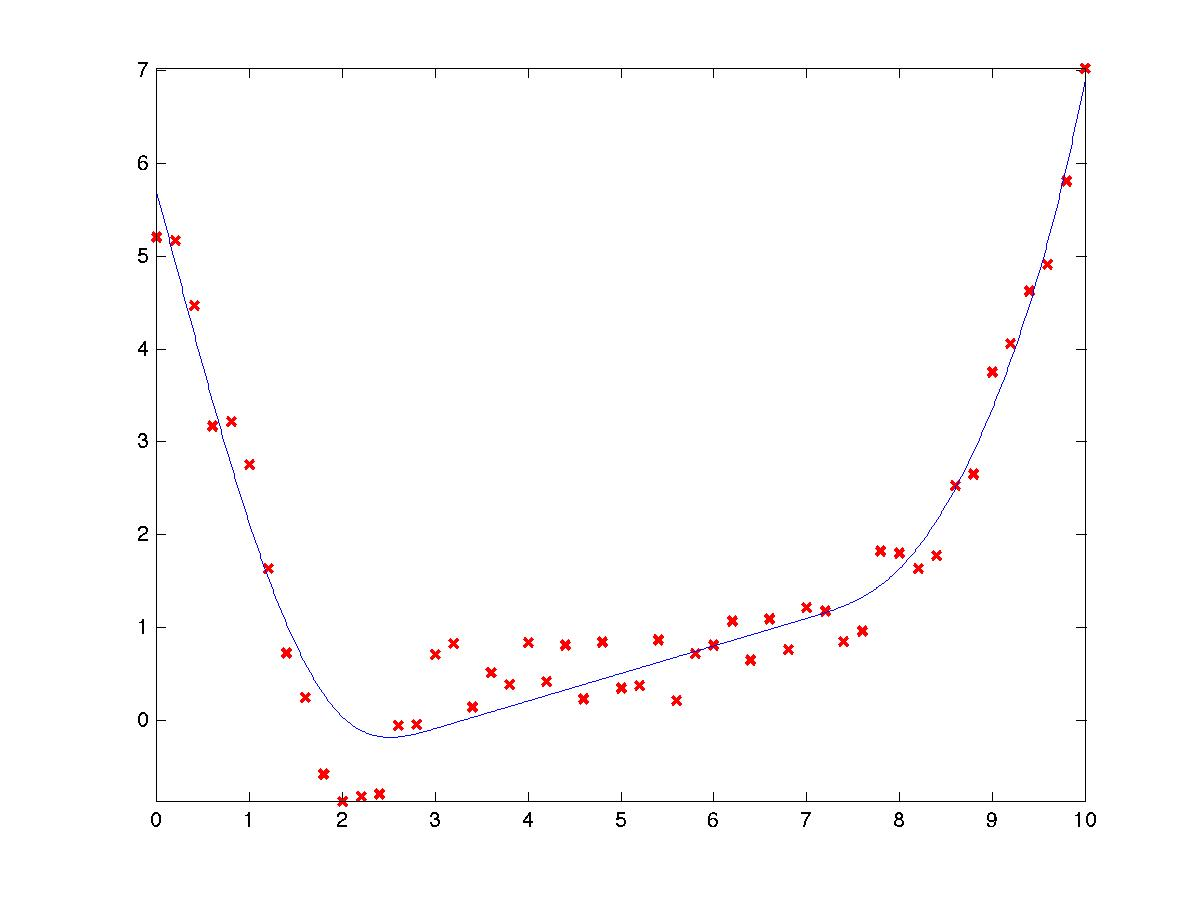
\includegraphics[scale=0.25]{hw2_p58_fit.jpg}
\end{center}
\begin{verbatim}
[t, y] = spline_data();
A = zeros(51,13);
G = zeros(51,13);
h = zeros(51,1);

for i=1:51
[y1,yp,ypp] = bsplines(t(i));
A(i,:) = y1';
G(i,:) = -ypp';
end

cvx_begin 
variable x(13)
minimize( (A*x-y)'*(A*x-y) )
subject to 
    G*x <= h
cvx_end

fit_x = linspace(0,10,1000);
fit_y = zeros(1,1000);
for i=1:1000
    fit_y(i) = x' * bsplines(fit_x(i));
end

plot(t,y,'rx', 'LineWidth', 2);
hold on
handle = plot(fit_x, fit_y, 'b-');
axis equal
saveas(handle,'EE236B_hw2_p58_fit','jpg');
hold off
\end{verbatim}


\end{document}
